\documentclass[a4paper]{article}
\usepackage{graphicx}
\graphicspath{ {./img/} } % Required for inserting images
\usepackage[czech]{babel}
\usepackage[T1]{fontenc}
\usepackage[utf8]{inputenc}
\usepackage[top=1.5 cm, left=1.5 cm, right=15mm, bottom=15mm]{geometry}
\usepackage{fancyhdr, color, multicol}
\usepackage{ragged2e}
\usepackage{blindtext}
\usepackage{lipsum}
\usepackage{multicol}
\usepackage{tikz}
\usepackage{color}
\usepackage[fontsize=12pt]{fontsize}
\usepackage{circuitikz} %obvody, znacky
\usetikzlibrary{arrows}
\usepackage{tkz-euclide}
\usepackage{hyperref}
\hypersetup{
    colorlinks=true, %set true if you want colored links
    linktoc=all,     %set to all if you want both sections and subsections linked
    linkcolor=black,  %choose some color if you want links to stand out
}
%==========================Fonts=====================================
\usepackage{lmodern}
\rmfamily
\DeclareFontShape{T1}{lmr}{b}{sc}{<->ssub*cmr/bx/sc}{}
\DeclareFontShape{T1}{lmr}{bx}{sc}{<->ssub*cmr/bx/sc}{}
%====================================================================
\begin{document}
\thispagestyle{empty}
\begin{center}
    \vspace*{5cm}
    {\huge{1. Architektura PC}} \par
    \vspace{15cm}
    {\large{lilman2727}} \par
    \vspace{3cm}
    {\url{https://github.com/lilman2727/Maturitni-Otazky}}
\end{center}


\newpage
\thispagestyle{empty}
\tableofcontents
\newpage

\section{Velice stručná historie}
    \subsection{Analytický stroj}
        Analytický stroj je návrh obecně použitelného mechanického počítače. Obsahoval aritmetickou jednotku, řídící tok s podmíněným větvením a cykly a integrovanou paměť. Je to první \textit{turingovsky úplný} počítač, což znamená, že by teoreticky dokázal vyřešit jakoukoliv úlohu za pomocí přesně definovaných kroků zapsaných přesně definovanými symboly (algoritmem).\par
        S návrhem přišel anglický matematik Charles Babbage v roce 1837. Babbage ho sám nikdy nedokončil. První obecný počítač bude postaven až po více než 100 letech.

    \subsection{Turingův stroj}
        Turingův stroj je teoretický počítač, popsaný matematikem Alanem Turingem v roce 1936. Stroj posouvá nekonečně dlouhou pásku dle daných pravidel. Stroj z této pásky může číst či do ní zapisovat. Je teoreticky schopen vyřešit libovolný problém podle algoritmu.
    \subsection{Bombe}
        Bombe byl elektromechanický počítač sestrojený Alanem Turingem za druhé světové války. Jeho cílem bylo dešifrovat tajné zprávy zašifrované pomocí německé Enigmy. Stroj jako takový simuloval 36 strojů Enigma, s celkem 108 rotory, každý simulující 1 rotor stroje Enigma. Bombe využil slabinu Enigmy -- vstupní písmeno se nikdy nerovnalo výstupnímu 
    \subsection{ENIAC}
        Z anglického \textit{Electronic Numerical Integrator and Computer} byl první programovatelný elektronkový počítač sestrojený v roce 1945 v USA. Jeho prvním úkolem bylo zjistit proveditelnost termojaderné zbraně. Pro své logické obvody používal elektronky, tedy vakuuové trubičky; takovéto počítače jsou označovány názvem \textit{počítače první generace}. Jeho nástupce, MANIAC byl prvním strojem, který porazil člověka ve hře podobné šachu, tzv. Los Alamos šachy, hrané na $6 \times 6$ šachovnici, tedy bez střelců.
    \subsection{UNIVAC}
        Z anglického \textit{UNIVersal Automatic Computer} byl první komerčně vyráběný počítač. Byl vyrobený v USA a na vývoji se podíleli vynálezci strojů ENIAC a MANIAC. Tento počítač je známý tím, že předpovědel vítězství Eisenhowera ve volbách v roce 1952. Stejně jako ENIAC a MANIAC používal pro své obvody elektronky.
    \subsection{IBM PC}
        Uvedený na trh v roce 1981, tento počítač odstartoval éru počítačů jak je známe dnes. Přinesl uživatelské rozhraní a časem i spoustu rozšiřujících karet. Díky vynálezu mikroprocesoru bylo možné razantně zmenšit velikost počítače -- odstupuje se od sálových počítačů. Dnešní počítače jsou jakýmisi praprapravnuky právě IBM PC, používal procesor Intel 8088, měl paměť RAM a podporoval diskety.

\newpage


\section{Architektura počítačů}
    \textit{Architektura počítače} je způsob realizace počítače. Zaměřuje se na návrh a konstrukci zařízení, která zpracovávají data. Zkoumá, jak pracuje CPU a jak přistupuje k paměti.
    \subsection{Von Neumannova architektura}
        Architektura popsaná americko-maďarským matematikem Johnem von Neumannem. Popisuje počítač, který má společnou paměť pro instrukce i data. Zpracování dat je \textit{sekvenční}, tj. instrukce se vykonají v přesném pořadí jedna za druhou. Von Neumannova architektura  popisuje řadič s aritmeticko-logickou jednotkou jako centrální procesorovou jednotku, která komunikuje s pamětí. \par
        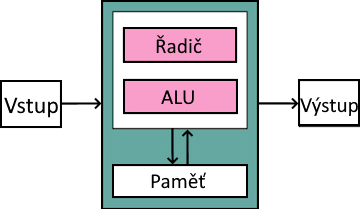
\includegraphics{vonNeumann.png}\par
        \captionsczech{Von Neumannova architektura, [1]}
    \subsection{Řadič}
        \textit{Řadič} řídí celou činnost počítače. Řadič v procesoru je nadřazen všem ostatním řadičům (např. paměťový řadič, SATA řadič\dots)
        Počítač řídí pomocí řídících signálů, které zasílá jednolivým modulům počítače a odpovědi na tyto signály jsou předány zpět do řadiče. \par
        V dnešní době používáme tzv. \textit{mikroprogramovatelné řadiče}, tedy řadiče řízené kódem, který je uložený v paměti. \par
        Existují tři typy mikroprogramovatelných řadičů:
        \begin{itemize}
            \item Horizontální -- používá dlouhé mikroinstrukce, které obsahují i řídící signály. Každá mikroinstrukce vyžaduje 1 takt. Mikroinstrukce obsahuje i adresu paměti.
            \item Vertikální -- používá krátké mikroinstruke, které však vyžadují více taktů.
            \item Diagonální -- kompromis mezi horizontálním a vertikálním. Jedna mikrointrukce vyžaduje 1 takt, ale neobsahuje adresu paměti, proto musí být přítomen i programový čítač.
        \end{itemize}
    \subsection{Aritmeticko-logická jednotka}
        \textit{Aritmeticko-logická jednotka}, neboli \textit{ALU} provádí logické (negace, konjunkce, disjunkce \dots) a aritmetické (sčítání, násobení, bitový posun \dots) operace s daty podle programu. ALU se používá výhradně pro celočíselné operace. Pro operace s plovoucí desetinnou čárkou se používá tzv. \textit{FPU}, neboli \textit{FLoating-Point Unit}, v češtině \textit{matematický koprocesor}. \par
        Největší velikost dat, se kterým ALU může pracovat se nazývá \textit{slovo}. Dnešní procesory (na architektuře x86-64) mají velikost slova 64 bitů.
    \subsection{Registry}
        \textit{Registr} je nejrychlejší paměť počítače, slouží pro uložení informace o velikosti jednoho slova. CPU používá registry pro práci s čísly a další zpracovávání informací. ALU a FPU mají své vlastní registry o své vlastní délce slova. Délka slova záleží na architektuře daného procesoru a instruknční sady, kterou procesor disponuje.
    \subsection{Sběrnice}
        \textit{Sběrnice}, anglicky \textit{bus} má za účel zajistit přenos dat a řídících povelů mezi dvěma a více elektronickými zařízeními. Přenos dat se řídí stanoveným protokolem -- určitým postupem jak a které informace si předat. V posledních letech se od sběrnic ustupuje ve prospěch dvoubodových spojů, na kterých, na rozdíl od sběrnice, jsou data přenášena bez potřeby adresy, čímž se uvolní místo pro jiná data, a navíší se tak výkon. Příkladem sběrnice je \textit{USB}, zkratka znamenající \textit{Universal Serial Bus}, či sběrnice \textit{PCI}. Příkladem dvoubodového spoje je moderní \textit{PCIe}.
    \subsection{Centrální procesorová jednotka}
        \textit{Centrální procesorová jednotka}, anglicky \textit{Central Processing Unit}, \textit{CPU} je souhrnné označení pro \textit{ALU, FPU, a řadič}. CPU umí vykonávat strojové instrukce a obsluhovat vstupy a výstupy. Na začátku bylo CPU složeno z mnoha individuálních částí, ale v 70. letech minulého století byly všechny části sloučeny do jednoho integrovaného obvodu. CPU, který má části sloučené do integrovaného obvodu se nazývá \textit{mikroprocesor}.
    \subsection{Harvardská architektura}
        Narozdíl od \textit{von Neumannovy} architektury odděluje Harvardská architektura paměť programu a dat. To znamená, že instrukce a programová data jsou uloženy zvlášť a nesdílí sběrnice. CPU může současně číst instrukci a zároveň přistupovat do paměti dat. Dochází tedy k paralelizaci a tudíž ke zvýšení výkonu oproti sekvenčnímu způsobu přístupu k datům von Neumannovy architektury.
        \par
        Dnešní procesory spojují tyto architektury dohromady. Uvnitř se chovají podle Harvardské architektury - oddělují paměť pro data a pro instrukce, ale zvenku se chovají podle von Neumannovy architektury, protože načítá data i program z hlavní paměti (RAM) najednou.
    \subsection{Mikroarchitektury}
        Představuje způsob, jakým je implementovaná instrukční sada v procesoru. Pro jednu danou instrukční sadu může existovat více mikroarchitektur, např. mikroarchitektura \textit{Zen} a mikroarchitektura \textit{Core} implementují instrukční sady x86-64.
        \par
        Hlavním prvkem mikroarchitektury je \textit{exekuční jednotka}, která zahrnuje ALU, FPU, jednotky pro adresování, jednotky pro předpovídání větvení a \textit{SIMD} (Single Instruction, Multiple Data).

\newpage


\section{Hardware počítače}
    \subsection{Procesor}
        Je \uv{mozek} počítače. Procesor postupně zpracovává jednotlivé instrukce programu. Moderní procesory jsou vyráběny z křemíkového substrátu (wafer). Na substrát jsou naneseny miliony nanoskopických tranzistorů. Procesor, který se dnes používá se nazývá \textit{mikroprocesor}, protože je celý uložený do pouzdra integrovaného obvodu. \par
        Dnes se výrobou procesorů zabývají firmy, z nichž jsou hlavní \textit{AMD, Intel, ARM, Nvidia, Apple, Qualcomm}. Intel je schopen i výroby svých mikroprocesorů, kdežto ostatní výrobci jsou odkázáni na dodavatele, jako například \textit{TSMC}.
        Procesor, který dnes používáme obsahuje krom jádra procesoru i integrovaný rozvaděč tepla, který výrazně napomáhá chlazení.
    \subsection{Chladiče}
        Většina elektrické energie dodávaná polovodičovým součástkám je přeměněna na teplo. Protože by se jednotlivé součástky mohly poškodit, je velmi důležité je adekvátně chladit. U procesorů dle \textit{TDP, Thermal Design Power} lze určit, jak moc \uv{budou hřát} a podle toho zvolit správný chladič. \par
        Chladiče můžeme rozdělit následovně:
        \begin{itemize}
            \item Pasivní chlazení -- teplo generované polovodičem se přesune na, většinou hliníkový, chladič, který si vyměňuje teplo s okolím. Pasivní chladiče se v drtivé většině dělají do $37\,W$, po překročení této hodnoty je skoro nutné přejít na aktivní chlazení.
            \item Aktivní chlazení -- lze rozlišit na:
            \begin{itemize}
                \item Chlazení vzduchem -- větrák fouká čerstvý vzduch do chladiče a tak značně pomáhá s rozptylem tepla. Krom větráku je identický s pasivním chladičem ve funkčnosti i v obecném principu funkčnosti.
                \item Chlazení vodou -- používá kapalinu, která proudí skrze uzavřený okruh přes procesor až k radiátoru, kde si s ním vymění teplo. Lze rozdělit na:
                \begin{itemize}
                    \item AIO -- All-in-one -- obsahuje chladící desku, pumpu, kapalinu, trubičky, radiátor a větráky na radiátor v jednom uceleném balení, \uv{plug and play}
                    \item Custom loop -- Všechny výše uvedené části a k tomu rezervoár (nádrž) si koupíte zvlášť a sestavíte se na míru dle svých požadovaných specifikací. Nutné značné úsilí, je dražší.
                \end{itemize}
            \end{itemize}
            \item Chlazení tekutým dusíkem -- v extrémních případech, tekutý dusík se nalévá přímo na jádro CPU/GPU. Velice nepraktické k dennímu použití, ale lze tak dosáhnout nejlepšího výkonu.
        \end{itemize}
    \subsection{Základní deska}
        Hlavní funkcí základní desky je propojit jednotlivé komponenty do fungujícího celku a poskytnout jim stabilní elektrické napájení. Funguje tedy jako jakási nervová soustava celého počítače -- jednotlivé komponenety by se bez ní nemohly domluvit. \par Na základní desce se nachází mimo níže popsané i např. BIOS čip, který se stará o základní nastavení desky. Jednotlivá uživatelská nastavení se nahrávají do volitilního (potřebuje stálý přísun elektrické energie, aby si pamatoval data), která je poháněna knoflíkovou baterií. \par
        Základní desku musíme vybrat podle procesoru, aby procesor pasoval do patice a byl podporován čipovou sadou.
        \par
        Existuje také několik formátů základních desek, mezi nejpoužívanější patří:
        \begin{itemize}
            \item ATX -- nejrozšířenější formát základních desek, měří $305 \times 244 mm$ (výška x šířka)
            \item E-ATX -- není formálně definovaný, ale E-ATX (Extended-ATX) je jakýsi souhrn standardů SSI CEB, SSI EEB a celkově jakéhokoli formátu přesahující šířku standardní ATX desky.
            \item microATX -- zmenšená ATX deska, měří $244 \times 244 mm$
            \item mini-ITX -- nejmenší formát základní desky běžně k dostání. Měří $170 \times 170 mm$.
        \end{itemize}
        \subsubsection{Patice}
            Patice, neboli \textit{socket}, je místo na fyzické propojení procesoru a základní desky. Patice byla vyvinuta pro možnost použít více procesorů na jedné základní desce. Pro zapojení do patice nepotřebujeme skoro žádnou sílu -- v případě správné orientace procesor zapadne vlastní tíhou. \par Rozlišujeme dva typy patic, dle způsobu kontaktu s procesorem:
            \begin{itemize}
                \item PGA -- \textit{Pin Grid Array} -- \textbf{procesor} má na sobě piny, které jsou uspořádány tak, aby seděly do otvorů v patici. Tohoto typu patice využívá např. Socket AM4, též známá pod názvem PGA-1331.
                \item LGA -- \textit{Land Grid Array} -- Kontaktní plošky na procesoru se dotýkají miniaturních pinů \textbf{v patici}. Tento typ patice využívá společnost Intel, např socket LGA-1700, či AMD s paticí AM5.
            \end{itemize}
            Před používáním patic bylo běžné mít procesor připájený přímo na základní desku s použitím \textit{BGA, Ball Grid Array}. BGA prakticky znemožňuje laikům vyměnit si procesor. BGA se dnes používá převážně pro notebooky či přenosná zařízení.
        \subsubsection{Čipová sada}
        \begin{multicols}{2}
                Čipová sada, neboli \textit{chipset} je sada specializovaných obvodů. Nejčastěji mívají na starost komunikaci s disky a USB. 
                \par
                Tradičně byl čipset rozdělený na dva -- \textit{North bridge} a \textit{South bridge}. North bridge obsluhoval převážně operační paměť a PCIe pro grafickou kartu, kdežto south bridge obsluhoval sběrnici SATA, USB, ostatní PCIe linky, SuperIO a BIOS čip. 
                \par
                V dnešní době je však north bridge zakomponován přímo do CPU. Dle architektury procesoru může procesor \uv{přebrat} další funkce od south bridge. Například procesory \textit{Ryzen} mají integrované obvody pro obsluhu SuperIO, některé USB a SATA. \par
                pozn.
                \begin{itemize}
                    \item  \textit{SuperIO} je série integrovaných obvodů, které obsluhují mmj. PS/2 porty pro klávesnici a myš, LED    diody, PWM signály pro větráky.
                    \item Můžeme se setkat i s názvem \textit{PCH}, znamenající \textit{Platform Controller Hub}. Jde o obchodní označení firmy Intel pro jednočipový čipset. 
                \end{itemize} 
                \vspace{48pt}
                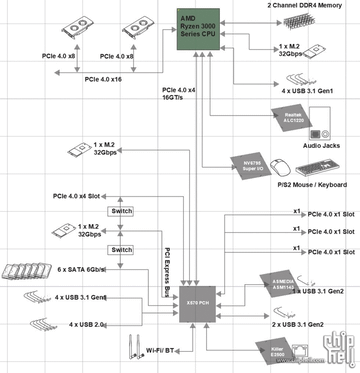
\includegraphics[scale=0.9]{img/chipset.png} \par
                \captionsczech{Chipset, [2]}
        \end{multicols}

        \subsubsection{Napájecí kaskády}
            Napájecí kaskády zajišťují aby se všem součástkám počítače dostavilo správné napájení. Různé součástky vyžadují rozdílné hodnoty napětí, aby správně fungovaly. (např. CPU potřebuje $1--1,5\,V$, větráky $12\,V$.) \par
            Napájecí kaskáda zahrnuje několik elektrotechnických součástek:
            \begin{itemize}
                \item \textit{MOSFETy} (\textit{Metal-Oxide-Semiconductor Field Effect Transistor}) -- regulují napětí.
                \item \textit{Tlumivky} -- čož jsou ve své podstatě cívky. 
                \item \textit{Kondenzátory} -- filtrují náhlé skoky či poklesy v napětí.
                \item \textit{ovladač kaskády} -- který řídí celou napájecí kaskádu
            \end{itemize}
            Tyto komponenty zajišťují, aby se každému komponentu dostalo adekvátní napětí, je proto důležité sáhnout po základní desce s kvalitní kaskádou.
        \subsubsection{Integrované technologie}
            V dnešní době je spousta technologií již zakomponována do základní desky. Nejsou tak potřeba rozšiřující karty na běžné užívání PC. Mezi technologie, které jsou integrované do základních desek považujeme:
            \begin{itemize}
                \item Zvuková karta
                \item Síťová karta
                \item Wi-Fi -- v některých případech, hlavně u základních desek formátu mini-ITX bývá standardem zabudovaná Wi-Fi.
                \item Bluetooth -- stejně jako Wi-Fi, i Bluetooth bývá zabudován do některých základních desek, obzvlášť formátu mini-ITX
            \end{itemize} \par
            pozn. Základní desky, které mají zabudovaný Bluetooth a Wi-Fi jsou často označovány písmeny AC. Např. \textit{Asus Crosshair VI Hero AC}.
        \subsubsection{Sběrnice, piny a jiné konektory}
            Základní deska disponuje mnoha konektory, mezi nejvýznamnější patří:
            \begin{itemize}
                \item RAM Sloty -- jak název napovídá, do těchto slotů se zapojuje operační paměť RAM. Je propojena přímo s CPU.
                \item PCIe -- \textit{Peripheral Component Interconnect Express} slouží pro připojování vysokorychlostních zařízení, jako například GPU či SSD. Nejmodernější verze je schopna průpostnosti $31,5\,GB/s$. Zařízení vyžadující vysokou propustnost se připojují do 16 linek PCIe, kdežto méně výkonným stačí linek 8, 4, 2 nebo i 1. Hovoříme pak např. o PCIe gen. 4 x16, kdy za slovíčkem gen uvádíme číslo generace a potom uvádíme počet linek v daném slotu. 
                \item SATA -- \textit{Serial AT Attachment} -- slouží výhradně pro připojování datových zařízení jako například SSD, HDD, optické disky \dots Dnes se pomalu od SATA ustupuje ve prospěch standardu m.2 na \uv{sběrnici} PCIe.
                \item USB -- \textit{Universal Serial Bus} -- slouží na připojování externích zařízení, asi nejznámější sběrnice na světě.
                \item LAN port -- slouží pro připojení počítače do sítě.
                \item Audio porty -- Nejčastěji ve formě $3,5mm$ jacků, na dražších deskách i \textit{S/PDIF}.
            \end{itemize}
    \subsection{RAM}
        \textit{RAM}, \textit{Random Access Memory}, neboli \textit{Paměť s náhodným přístupem} je vitální část počítače. V RAM se ukládají veškerá data programů, na kterých se zrovna pracuje. Jde o volatilní typ paměti, tedy potřebuje neustálý přístup eletřiny, jinak dojde ke ztrátě dat. V dnešní době se používá RAM typu DRAM, neboli dynamická RAM. Oproti starší SRAM (static RAM) má DRAM výhodu mnohem vyšší kapacity a vyšší energetické účinnosti.
        \subsubsection{Rozdíly mezi SDR, DDR, QDR}
            RAM existují ve třech \uv{příchutích} -- \textit{SDR}, \textit{DDR} a \textit{QDR}. Tyto typy RAM se liší podle počtu transferů v daném cyklu. Paměť typu SDR (\textit{Single Data Rate}) provede jeden transfer za cyklus. Paměť typu DDR (\textit{Double Data Rate}) provádí dva transfery za cyklus. Paměť typu QDR (\textit{Quad Data Rate}) provádí celkem 4 transfery za cyklus. \par
            Pro správnost by se tedy měl počet transferů uvádět v jednotce $MT/s$ -- mega transfery za sekundu, oproti reálnému taktu pamětí -- ten se uvádí v $MHz$ a je v případě DDR vždy o \textit{polovinu} menší.
    \subsection{Grafická karta}
        Je zařízení, které se stará o zobrazování obrazu na monitoru. Je specializovaná na vysoce paralelní, relativně lehké operace (vektorové operace, maticové operace, aritmetika\dots). Narozdíl od procesoru obsahuje tisíce jader, která spolu pracují na dané práci zároveň. Díky tomuto je grafická karta extrémně rychlá v relativně úzkém okruhu problémů, avšak problémy vyžadující paralelizaci jsou na GPU několikanásobně rychlejší než na CPU. \par
        Grafické karty můžeme rozdělit na dedikované a integrované. Integrované grafické karty se nacházejí přímo v procesoru. Mají výhodu malé energetické náročnosti, avšak nejsou schopny takového výkonu jako karty dedikované. Oproti tomu, dedikované grafické karty obsahují své vlastní obvody a komunikují s procesorem pomocí dvoubodového spoje PCIe. Jsou větší, energeticky náročnější, ale jsou mnohem výkonnější.
        \subsubsection{Jádro a VRM}
            Jádro grafické karty tvoří GPU - \textit{Graphics Processing Unit}. To je tvořeno několika tisíci tzv. \textit{Stream procesorů} v případě AMD anebo \textit{CUDA jádry} v případě Nvidia. Jejich počet ovlivňuje výkon grafické karty. \par
            Dedikovaná grafická karta disponuje vlastní napájecí kaskádou, je tedy v tomto ohledu nezávislá na kaskádě základní desky.
        \subsubsection{Paměť GPU}
            V případě grafické karty integrované sdílí GPU operační paměť s CPU. Oproti paměti dedikované karty je operační paměť pomalá. Její velikost se většinou dá nastavit v UEFI/BIOSu. \par
            Dedikovaná grafická karta má i svou vlastní paměť, nazývanou VRAM, \textit{Video RAM}. RAM je přímo připájená na tištěný obvod a umožňuje současný zápis a čtení, proto se setkáváme s označením GDDR -- \textit{Graphics Double Data Rate}. U high-endových grafických karet se můžeme setkat s označením např. GDDR5X -- X znamená, že se jedná o paměť typu QDR, ale kvůli horší výslovnosti se zanechal technicky \uv{špatný} název GDDR (oproti GQDR). \par
            Dalším zajímavým typem paměti je \textit{HBM}, \textit{High Bandwidth Memory}, neboli \textit{vysokovýkonnostní paměť}. Te se používá pro extrémně výkonné grafické karty a je připájená přímo na substrát jádra grafické karty. Použila se také pro výrobu grafických karet Radeon R9 Fury a série Vega. Kvůli vysoké ceně se upřednostňuje grafická paměť GDDR.
    \subsection{Disky}
        Diskem se rozumí typ nevolatilní paměti, tedy typ paměti uchovávající data po přerušení dodávky elektřiny, který se používá pro dlouhodobé uložení dat. Oproti pamětem typu RAM jsou disky pomalejší, ale mají měkolikanásobnou velikost. V dnešní době se převážně používá disk typu SSD. Běžně se připojují pomocí sběrnice SATA či pomocí dvoubodového spoje PCIe.
        \subsubsection{HDD}
            \textit{HDD}, \textit{Hard Disk Drive}, neboli \textit{pevný disk} je typ magnetického disku, který pro zapisování dat používá pohyblivou hlavičku, pomocí které se magnetizují mikroskopické buňky. Hlavička je pak schopna data přečíst nebo data přepsat. Tyto hlavičky se hýbou nad točícím se \uv{kruhem}. Rychlost otáčení závisí na disku, ale většinou je pro desktop 7200 ot/min a pro notebooky 5400 ot/min. Pro urychlení přístupu často obsahují i cache, která přednačítá data.
        \subsubsection{SSD}
            \textit{SSD}, \textit{Solid State Drive}, neboli \textit{polovodičový disk} je typ disku, který nemá žádné pohyblivé části. Je tak mnohem odolnější proti nárazům. Pro ukládání dat používá nevolatilní paměť flash. Jsou mnohem rychlejší než klasické HDD a cenově se velmi přibližují HDD, proto se ve většině případech upřednostňuje SSD. Jedinou nevýhodou je životnost, udávaná v \textit{TBW}, \textit{TerraBytes Written}, a proto se v případech, kdy dochází k častému přepisu dat, upřednostňují HDD.
        \subsubsection{Archaické disky}
            Tyto disky již dnes, až na výjimky, nepoužíváme. Jde o \textit{floppy disky}, známé pod názvem \textit{diskety}. Dalším příkladem jsou magnetické pásky, CD a DVD, a HDD s konektory PATA.
    \subsection{Zdroj}
        Zdroj je součástka, která převádí ze střídavého napětí na napětí stejnosměrné. To dělá díky řadě interních komponentů. Zdroj je velice důležitá část počítače a špatný výběr zdroje může skončit i požárem. Zdroj  dodává celému počítači elektrickou energii, díky které může počítač pracovat. Zdroje se vyrábí s výkonem od $300\,W$ do $1600\,W$. Zdroje mají několik velikostí, z čehož nejhlavnější jsou ATX, SFX a SXF-L.
        \subsubsection{Hodnocení zdrojů}
            Existuje systém hodnocení, který udává, jakou účinnost má daný zdroj při různých úrovních zátěže, typicky $0\%, 50\% a 100\%$. Tento systém však nezaručuje kvalitu zdroje. Existují následující úrovně účinnosti: Bronze, Silver, Gold, Platinum, Titanium.
    \subsection{Rozšiřující karty}
        Jak již název napovídá, rozšiřující karty rozšiřují konektivitu PC. Existují např. USB karty, síťové karty, Wi-Fi karty, zvukové karty, aj. Tyto karty nejsou třeba k chodu PC a jsou mnohdy integrované přímo do základní desky. Jejich účelem je nabídnout spotřebiteli možnost rozšířit si počítač o příslušné funkce.
    \subsection{Bedny}
        Uceluje celou sestavu. Teoreticky není potřebná k chodu PC. Obsahuje externí konektory, jako např. USB či audio. Dále má i tlačítko na zapnutí PC. Bedny umožnují osazení větráků, radiátorů či jiných chladičů do ideálních poloh. \par
        Bedny se dají podle velikosti rozdělit na, od vzestupné velikosti: Mini-Tower, Mid-Tower, Full-Tower, HPTX. Toto rozdělení však nemá formální definici, a tak je důležité se dívat na reálné rozměry bedny a typy základních desek, které podporují.


\newpage

\section{Reference}
    \begin{itemize}
        \item \url{https://en.wikipedia.org/wiki/MANIAC_I}
        \item \url{https://en.wikipedia.org/wiki/IBM_Personal_Computer}
        \item \url{https://en.wikipedia.org/wiki/UNIVAC_I}
        \item \url{https://cs.wikipedia.org/wiki/ENIAC}
        \item \url{https://cs.wikipedia.org/wiki/Elektronkov%C3%BD_po%C4%8D%C3%ADta%C4%8D}
        \item \url{https://en.wikipedia.org/wiki/Bombe}
        \item \url{https://cs.wikipedia.org/wiki/Turingovsk%C3%A1_%C3%BAplnost}
        \item \url{https://cs.wikipedia.org/wiki/Turing%C5%AFv_stroj}
        \item \url{https://en.wikipedia.org/wiki/Turing_machine}
        \item \url{https://cs.wikipedia.org/wiki/%C5%98adi%C4%8D}
        \item \url{https://cs.wikipedia.org/wiki/%C4%8C%C3%ADta%C4%8D_instrukc%C3%AD}
        \item \url{https://cs.wikipedia.org/wiki/Architektura_po%C4%8D%C3%ADta%C4%8De}
        \item \url{https://en.wikipedia.org/wiki/Processor_register}
        \item \url{https://cs.wikipedia.org/wiki/Aritmeticko-logick%C3%A1_jednotka}
        \item \url{https://cs.wikipedia.org/wiki/Von_Neumannova_architektura}
        \item \url{https://cs.wikipedia.org/wiki/Sb%C4%9Brnice}
        \item \url{https://cs.wikipedia.org/wiki/PCI-Express}
        \item \url{https://cs.wikipedia.org/wiki/Centr%C3%A1ln%C3%AD_procesorov%C3%A1_jednotka}
        \item \url{https://cs.wikipedia.org/wiki/Harvardsk%C3%A1_architektura}
        \item \url{https://cs.wikipedia.org/wiki/Architektura_po%C4%8D%C3%ADta%C4%8De}
        \item \url{https://cs.wikipedia.org/wiki/Mikroarchitektura}
        \item \url{https://cs.wikipedia.org/wiki/Mikroprocesor}
        \item \url{https://cs.wikipedia.org/wiki/Patice_procesoru}
        \item \url{https://en.wikipedia.org/wiki/CPU_socket}
        \item \url{https://www.alza.cz/co-je-zakladni-deska}
        \item \url{https://en.wikipedia.org/wiki/ATX}
        \item \url{https://en.wikipedia.org/wiki/PCI_Express}
        \item \url{https://en.wikipedia.org/wiki/Random-access_memory}
    \end{itemize}
\section{Zdroje obrázků}
    \begin{itemize}
        \item[1.] \url{https://cs.wikipedia.org/wiki/Von_Neumannova_architektura}
        \item[2.] \url{https://www.guru3d.com/story/amd-x570-chipset-blockdiagram-surfaces-shows-specs} 
    \end{itemize}
\end{document}